\documentclass[USenglish]{ifimaster}

\usepackage[utf8]{inputenc}
\usepackage{ifikompendiumforside}
\usepackage{graphicx}
\usepackage[acronym]{glossaries}
\usepackage[backend=biber,sorting=none]{biblatex}

\usepackage{tabularx}
\usepackage{cleveref}

\makeglossaries

% Acronyms
\newacronym{dil}{DIL}{Disconnected, Intermittent and Limited environments}
\newacronym{nec}{NEC}{Network Enabled Capability}
\newacronym{soa}{SOA}{Service-Oriented Architecture}

\title{Improving the performance of Web Services in Disconnected, Intermittent
and Limited Environments}
\author{Joakim Johanson Lindquister}
\bibliography{references}

\begin{document}
\ififorside{}

\chapter*{Abstract}
In this thesis I investigate different techniques to improve the performance of
Web services in typical tactical network environments.
\pagebreak

\tableofcontents
\listoftables
\listoffigures

\pagebreak


\chapter{Introduction}
Military units may operate under conditions where the reliability of the network
connection is low. They can operate far from existing communication
infrastructure and rely only on wireless communication. Such networks are often
characterized by unreliable connections with low bandwidth and high error rates
making data communication difficult. In a military scenario it is necessary for
units at all operational levels to seamlessly exchange information across
different types of communication systems. To NATO, this concept is referred to
as \gls{nec}. In a feasibility study, NATO identified the \gls{soa} and Web
Services as key enablers\cite{nnec-study}.

Web services are well tested in civil environments where the network is stable
and the bandwidth is abundant. However, military networks may suffer
from high error rates and low bandwidth which can leave the Web services
unusable. In this thesis I investigate how these challenges can be overcome by applying optimization techniques at different layers of the protocol stack.
%Ikke ta for gitt at sensor vet hva protocol stack er? Kanske forenkle eller utdype

\section{Background and Motivation}
NATO is a military alliance consisting of 28 member
countries\cite{nato-homepage-member-countries} and which primary goal is to
protect the freedom and security of its members through political and military
means. In joint military operations the relatively large number of member
countries can be a challenge when setting up machine-to machine information
exchange. Differences in communication systems and equipment can attribute to
make data communicating difficult. In order to address this issue, NATO has
chosen the \gls{soa} concept\cite{IST-090}.

\subsection{Service-Oriented Architecture}
\glsentryfull{soa} is an architectural pattern where application components
provide services to other components over a network. \gls{soa} is built on
concepts such as object-orientation and distributed computing and aims to get
a loose coupling between clients and services. In their reference model for
\gls{soa}\cite{oasis-soa-reference-model}, the Organization for the Advancement
of Structured Information Standards (OASIS) define \gls{soa} as: \paragraph{}
\textit{Service Oriented Architecture is a paradigm for organizing and utilizing
distributed capabilities that may be under the control of different ownership
domains. It provides a uniform means to offer, discover, interact with and use
capabilities to produce desired effects consistent with measurable preconditions
and expectations.} % SOA Trekant figur her

\paragraph{}
 In \gls{soa} business logic is divided into smaller chunks of logic,
referred to as \textit{services}. A service can be business related, e.g a
patient register service, or a infrastructure service used by other services and
not by a user application.  Services are provided by \textit{service providers}
and are consumed by \textit{service consumers}. The service provider is
responsible for creating a service description, making the service available to
others and implementing the service according to the service description.
Services are made available through a \textit{service registry}, where service
providers publish service descriptions. Service consumers find the services they
need by contacting the service registry. The communication between services
occur through the exchange of standardized messages.

Following the \gls{soa} principles dictates a loose coupling between services
and service consumers which allows software system to be more flexible. Loose
coupling with regards to time enables services and its consumers to not be
available at the same instance of time. This enables asynchronous communication.
Loose coupling with regards to location allows the location of an service to be
changed without needing to reprogram, reconfigure, or restart the service
consumers. This is possible through the usage of the service registry, which is
updated with the new location.

Furthermore SOA enables service implementation neutrality. The implementation of
service is completely separated from the service description. This allows
re-implementation and alteration of a service without affecting the service
consumers. Thus this can attribute to keep development costs low and avoiding
proprietary solutions and vendor lock-in. Another benefit with SOA is
reusability by dividing common business processes into services, which may help
cost reduction and avoids duplication.

\gls{soa} is only a pattern and the concepts can be realized by a range of
technologies. The most common used approach is the Web service familiy of
standards, using the SOAP messaging protocol. To achieve interoperability
between systems from different nations and vendors, NATO has chosen the Web
service technology in order to realize the SOA principles. This allows member
nations to implement their own technology as long as they adhere to the
standards. Web services are are discussed in detail in \cref{web-services}.

\subsection{Military Networks}
% Trenger mer kjøtt her.
Web services can be used in strategic military networks as they have network
infrastructure with the same characteristics as civil networks.

\subsubsection{Tactical Networks}
Mobile tactical networks are characterized by that the units use tactical
communication equipment which includes technologies like VHF, UHF, HF,
tactical broadband and satellites. Examples of such units are mobile units
like vehicles, foot soldiers and field headquarters. These types of networks
have low bandwidth, possibly high delay, high error rates and frequent
disconnections. They are often called disadvantaged grids or DIL. NATO studies
has identified such networks to have the following characteristics:

\textit{
Disadvantaged grids are characterized by low bandwidth,variable throughput,
unreliable connectivity, and energy constraints imposed by the wireless
communications grid that link the nodes}\cite{nato-disadvantaged-grids}.
\paragraph{}
The characteristics of these networks and what challenges they impose are
discussed in detail in \cref{dil}.

\section{Problem Statement}
Most of the Web Service solutions used today are aimed for civilian use and does
not necessarily perform well in military environments. In contrast to civilian
networks where bandwidth are abundant, mobile tactical networks may suffer from
high error rates and low bandwidth. Adapting Web service solutions meant for
civil networks directly for military purposes may not be possible. Therefore,
Web services needs to be adapted in order to handle network challenges. However,
it can be very expensive to alter existing Web service technology and incoperate
proprietary solutions. A NATO research task group has previously identfied the
foundation on open standards to avoid tighter coupling between service providers
and consumers\cite{IST-090}. It is much better to use commercial off-the-shelf
software. By placing the optimization in proxies, the Web services can remain
unchanged.

The goal of this thesis is to investigate different optimization techniques that
can be applied in order to improve Web service performance in disadvantaged
networks. In order for the clients and services to remain interoperable the
optimization techniques will be placed in proxies. The Web Services will
communicate as normal, while all network traffic is tunneled through a proxy.
The Web Service itself does not need to pay attention to the bad connectivity,
the proxy will choose the appropriate protocol and configuration.

\section{Premises}
The Web services does not need to be changed.

\section{Scope and Limitations} Snevre inn oppgaven.

\section{Research Methodology}
Denning.

\section{Contribution}
The outcome of this thesis is an recommandation regarding which optimizations
techniques which can be used in DIL to enhance the performance of Web services.
\section{Outline}
Hvordan er resten av oppgaven strukturert.


%%%%% BACKGROUND %%%%
\chapter{Background}
In this part, I will present relevant technologies.
\section{Related Work}
Diskuterer eksisterende arbeid.



%%%%%%% WEB SERVICES
\section{Web services}
\label{web-services}
Web services are client and server applications that communicate over a network
and can be used to implement a service-oriented architecture. There exists many
definitions of Web services where the core principles are the same, but the
finer details may vary. The World Wide Web Consortium has defined Web Services
as\cite{wrc-web-service}:
\paragraph{}
\textit{
    A Web service is a software system designed to support interoperable
    machine-to-machine interaction over a network. It has an interface described in
    a machine-processable format (specifically WSDL). Other systems interact with
    the Web service in a manner prescribed by its description using SOAP-messages,
    typically conveyed using HTTP with an XML serialization in conjunction with
    other Web-related standards.
}

\paragraph{}
This definition points out a set of standards that enables machine-to-machine
interactions. These standards are discussed in the following sections.
Figur her.

\subsection{XML}
Extensible Markup Language(XML) is a markup language and is considered as the
base standard for Web services. An XML document consist of data surrounded by
tags and is designed to be both machine and user readable. In a Web service, XML
is used to tag the data. 
\subsection{Service descriptions: WSDL}
Web Services Description Language(WSDL) is an interface definition language that
using XML describes functionality offered by a Web service. The interface
describes available functions, data types for message requests and responses and
binding information about the transport protocol, as well as address information
for locating the service.
\subsection{SOAP}
SOAP is an application level XML based protocol specification for information
exchange in the implementation of Web services. It is transport protocol
agnostic and can be carried over various protocols. The far most used is HTTP
over TCP, but other protocols such as UDP and SMTP can be used as well.
A SOAP message consist of a optional header and a required body. The header can
contain information not directly related to the message, such as routing
information for the message. The body contains the data being sent, known as the
payload.
\subsection{Other Web services}
However, there also exist other types of Web services which does not follow the
previously discussed standards. RESTful web services let users manipulate data
using a set of stateless operations. It uses exclusively HTTP. REST services are
easy to understand and have gained a lot of traction in the civil industry in
the latest years.


%%%%%%%%%% DIL %%%%%%%%%%%%%%%
\section{DIL}
\label{dil}
\paragraph{}
These constrains of mobile tactical networks are central in order to understand
the problem at hand, and I will therefore explain the concepts here:
\begin{description}
\item[Bandwidth and throughput] The terms bandwidth and throughput are used
interchangeably in the networking community and refers to the data transfer
rate; how fast data can be transported from one point to another in given time
period. This is often expressed in bits per second.
\item[Unreliable connectivity] Units that are participating in a tactical
network are highly mobile and may disconnect from a network either voluntarily
or not. Unplanned loss of connectivity can be due to various reasons, such as
loss of signal or equipment malfunction.
\item[Energy constraints imposed by the wireless communication grid] The battery
capacity and the transmission range of the communication equipment for mobile
units may be limited. Another issue is that in some cases military units are
required to enter radio silence in order to avoid being detected by the enemy.
During radio silence units may only receive data and not send any.
\end{description}

These constrains impose some challenges when employing Web services in
tactical networks. In a paper, tree areas that need to be addresses are
identified\cite{IST-118}.
\label{section:DIL-problems}

\subsubsection{End-to-end connections}
Attempting to establish and maintaining connections in DIL environments can lead
to increased communication overhead and possible complete breakdown of
communication. \subsubsection{Network heterogeneity}
Different technologies used. Different performance in networks may lead to
buildup of data in buffers, risking loss of information.
\subsubsection{Web Service overhead}
Web services generate overhead.
\section{Optimization techniques}
Web services enables interoperability betweens system, but also increase the
information overhead, requiring higher data rate demands. By using proxies, we
can freely choose the communications protocols and configurations between the
proxy pair without altering the Web Services themselves. In this thesis I will
investigate different techniques in order to optimize the communication between
a Web Service and a Web Service client. The optimization can be implemented at
different levels of the protocol stack in use.
\Cref{table:optimalization-overview} lists an overview of possible optimization
techniques studied in this thesis. \\ \\

%%%%%%%% TABLE OPTIMALIZATION OVERVIEW %%%%%%%%%%%%%
\begin{table}[h]
\begin{tabularx}{\textwidth}{| X | X |}
\hline
  \textbf{Protocol Stack} & \textbf{optimization possibilities} \\ \hline
  The application & Optimize the application\\ \hline
  Web service messaging: SOAP & Optimize SOAP, e.g XML compression \\ \hline
  HTTP/TCP, UDP or other transport protocols & SOAP is transport agnostic. Other
  protocols can be used. \\ \hline
  IP & NATO NEC feasibility study states that all protocols should be over IP. \\
  \hline
  Lower layers & Not in the scope of this thesis. \\ \hline
\end{tabularx}
\caption{Optimization possibilities.} \label{table:optimalization-overview}
\end{table}


\subsection{Compressing the payload}
The first optimization techniques deals with the optimization of the encoding. By compressing the Web service payload, we can reduce the amount of data that need to be sent.
\begin{itemize}
\item GZIP
\item EFX(Efficient XML).
\end{itemize}
Previous experiments shows EFX has the compression results with GZIP as the second best alternative\cite{johnsen-trude-compression-techniqes}.

\subsection{Reducing overhead of SOAP}
HTTP/TCP is the most used transport protocol for SOAP messages, but since SOAP is transport protocol agnostic different protocols can be used. Experiments show that this is possible.


%%%%%%%%%%%% Transport protokoller %%%%%%%%%%%%%%%%%%%
\begin{table}[h]
\begin{tabularx}{\textwidth}{| X | X |}
\hline
  \textbf{Transport Protocol} & \textbf{Summary} \\ \hline
  HTTP over TCP & Widely used. Breaks down in DIL environments.\\ \hline
  Military Message Handling System(MMHS) & Optimize the application\\ \hline
  Stream Control Transmission Protocol(SCTP) & Features multihoming. \\ \hline
  Advanced Message Queuing Protocol(AMPQ) & Application level protocol. Employs
  a broker architecture with store-and-forward capabilities. \\ \hline
  SOAP directly on TCP & Its possible \\ \hline
\end{tabularx}
\caption{Transport protocols}
\end{table}

\section{Proxies}
A proxy is a server that acts as intermediary for requests between a client and
server over a network. Proxies can be used to accomplish different tasks, from
caching web content to bypassing filtering and censorship. We can group proxies
into three types, forwarding proxies, reverse proxies and gateway proxies.
\section{Requirement Analysis}
A discussed in \cref{section:DIL-problems}, the dependency on end-to-end
connections needs to be removed. This can be done by adding proxies to the
network. Mobile units have to carry batteries with them and the capacity is
therefore limited. Advanced compression techniques may reduce the overhead, but
also requires more battery. This trade-off needs to be considered.
\\ \\ \\
\begin{table}[h]
\begin{tabular}{| l | l |}
\hline
  \textbf{Requirement} & \textbf{Priority} \\ \hline
  Receive and forward HTTP 1.X requests & 1\\ \hline
  Allow modifications on the payload & 1 \\ \hline
  Allow configuration of HTTP timeouts & 1 \\ \hline
  Keep HTTP-connection alive & 1 \\ \hline
  Support protocol X and y & 2 \\ \hline
\end{tabular}
\caption{Proxy requirements}
\end{table}

\section{Summary}



%%%% Design and implementation %%%%
\chapter{Design and Implementation}
\section{Overall Design}
\section{Proxy}
\subsection{Squid}
Squid is a fully-featured HTTP/1.0 proxy.
\begin{figure}[h]
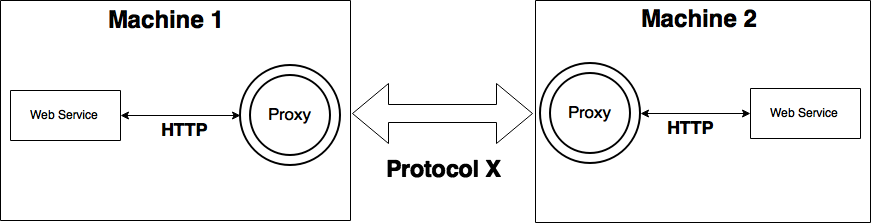
\includegraphics[scale=0.4]{images/architecture.png}
\caption{Architectural overview of proposed design}
\end{figure}



\subsection{Tuning application server configuration}

\subsection{Alternative transport protocols}

\section{Summary}

\chapter{Testing and Evaluation}
\section{Evaluation Tools}

\chapter{Conclusion and Future Work}
\section{Conclusion}

\section{Future Work}

\pagebreak
\printbibliography{}
\printglossary

\end{document}
